%%% MATH110-PS021-Solutions.tex --- 
%% 
%% Filename: MATH110-PS021-Solutions.tex
%% Description: 
%% Author: U-ORONYA\edwar
%% Maintainer: 
%% Created: Sun Jan 29 21:34:17 2023 (-0600)
%% Version: 
%% Package-Requires: ()
%% Last-Updated: Sun Jan 29 23:34:38 2023 (-0600)
%%           By: U-ORONYA\edwar
%%     Update #: 39
%% URL: 
%% Doc URL: 
%% Keywords: 
%% Compatibility: 
%% 
%%%%%%%%%%%%%%%%%%%%%%%%%%%%%%%%%%%%%%%%%%%%%%%%%%%%%%%%%%%%%%%%%%%%%%
%% 
%%% Commentary: 
%% 
%% 
%% 
%%%%%%%%%%%%%%%%%%%%%%%%%%%%%%%%%%%%%%%%%%%%%%%%%%%%%%%%%%%%%%%%%%%%%%
%% 
%%% Change Log:
%% 
%% 
%%%%%%%%%%%%%%%%%%%%%%%%%%%%%%%%%%%%%%%%%%%%%%%%%%%%%%%%%%%%%%%%%%%%%%
%%
%% Copyright (C) 2023 Edward Doolittle
%% 
%%%%%%%%%%%%%%%%%%%%%%%%%%%%%%%%%%%%%%%%%%%%%%%%%%%%%%%%%%%%%%%%%%%%%%
%% 
%%% Code:


\documentclass{article}
\usepackage{amsmath}
\usepackage{fullpage}
%\usepackage{graphicx}
\usepackage{tikz,pgfplots}
\pgfplotsset{compat=1.13}
% \allowdisplaybreaks
\usepackage[aux]{rerunfilecheck}

\newcommand{\ds}{\displaystyle}

% Macros for MATH 110 course dates

\newcommand{\commonTheme}{metropolis}
\newcommand{\commonColorTheme}{metropolis}

\newcommand{\commonAuthor}{Edward Doolittle}
\newcommand{\commonInstitute}{Department of Indigenous Knowledge and
  Science \\ First Nations University of Canada}
\newcommand{\commonCourse}{MATH 110 Calculus I}
\newcommand{\commonTerm}{202510}
\newcommand{\commonDate}{January 6, 2025}

% Review Material

% Lab 0
\newcommand{\commonEventNegativeOne}{LabNegativeOne}
\newcommand{\commonDateLabNegativeOne}{Monday, January 6, 2025}
\newcommand{\commonTitleLabNegativeOne}{MATH 110 Lab 0}
\newcommand{\commonSubtitleLabNegativeOne}{No Lab; Course Opens}

% Section 001
\newcommand{\commonEventZeroZeroOne}{ZeroZeroOne}
\newcommand{\commonDateZeroZeroOne}{Tuesday, January 7, 2025}
\newcommand{\commonTitleZeroZeroOne}{MATH 110 Review 0.1}
\newcommand{\commonSubtitleZeroZeroOne}{Review of Algebra}
\newcommand{\commonPSTitleZeroZeroOne}{MATH 110 Review Problem Set 0.1}

% Section 00A
\newcommand{\commonEventZeroZeroA}{ZeroZeroA}
\newcommand{\commonDateZeroZeroA}{Tuesday, January 7, 2025}
\newcommand{\commonTitleZeroZeroA}{MATH 110 Review 0.A}
\newcommand{\commonSubtitleZeroZeroA}{Review of Inequalities and
  Absolute Values}
\newcommand{\commonPSTitleZeroZeroA}{MATH 110 Review Problem Set 0.A}

% Section 00B
\newcommand{\commonEventZeroZeroB}{ZeroZeroB}
\newcommand{\commonDateZeroZeroB}{Tuesday, January 7, 2025}
\newcommand{\commonTitleZeroZeroB}{MATH 110 Review 0.B}
\newcommand{\commonSubtitleZeroZeroB}{Review of Coordinate Geometry
  and Lines}
\newcommand{\commonPSTitleZeroZeroB}{MATH 110 Review Problem Set 0.B}

% Section 00C
\newcommand{\commonEventZeroZeroC}{ZeroZeroC}
\newcommand{\commonDateZeroZeroC}{Thursday, January 9, 2025}
\newcommand{\commonTitleZeroZeroC}{MATH 110 Review 0.C}
\newcommand{\commonSubtitleZeroZeroC}{Review of Graphs of Second
  Degree Equations}
\newcommand{\commonPSTitleZeroZeroC}{MATH 110 Review Problem Set 0.C}

% Section 00D
\newcommand{\commonEventZeroZeroD}{ZeroZeroD}
\newcommand{\commonDateZeroZeroD}{Thursday, January 9, 2025}
\newcommand{\commonTitleZeroZeroD}{MATH 110 Review 0.D}
\newcommand{\commonSubtitleZeroZeroD}{Review of Trigonometry}
\newcommand{\commonPSTitleZeroZeroD}{MATH 110 Review Problem Set 0.D}

% Section 011
\newcommand{\commonEventZeroOneOne}{ZeroOneOne}
\newcommand{\commonDateZeroOneOne}{Thursday, January 9, 2025}
\newcommand{\commonTitleZeroOneOne}{MATH 110 Review 1.1}
\newcommand{\commonSubtitleZeroOneOne}{Review of Functions}
\newcommand{\commonPSTitleZeroOneOne}{MATH 110 Review Problem Set 1.1}


% Main Course

% Lab 1
\newcommand{\commonEventZero}{LabZero}
\newcommand{\commonDateLabZero}{Monday, January 13, 2025}
\newcommand{\commonTitleLabZero}{MATH 110 Lab 1}
\newcommand{\commonSubtitleLabZero}{Quiz 0: STACK, Onboarding}

% Section 1.4
\newcommand{\commonEventOne}{ZeroOneFour}
\newcommand{\commonDateZeroOneFour}{Tuesday, January 14, 2025}
\newcommand{\commonTitleZeroOneFour}{MATH 110 Lecture 1.4}
\newcommand{\commonSubtitleZeroOneFour}{The Tangent and Velocity Problems}
\newcommand{\commonPSTitleZeroOneFour}{MATH 110 Problem Set 1.4}

% Section 1.5
\newcommand{\commonEventTwo}{ZeroOneFive}
\newcommand{\commonDateZeroOneFive}{Thursday, January 16, 2025}
\newcommand{\commonTitleZeroOneFive}{MATH 110 Lecture 1.5}
\newcommand{\commonSubtitleZeroOneFive}{The Limit of a Function}
\newcommand{\commonPSTitleZeroOneFive}{MATH 110 Problem Set 1.5}

% Lab 2
\newcommand{\commonEventThree}{LabOne}
\newcommand{\commonDateLabOne}{Monday, January 20, 2025}
\newcommand{\commonTitleLabOne}{MATH 110 Lab 2}
\newcommand{\commonSubtitleLabOne}{Quiz 1: Review}

% Section 1.6
\newcommand{\commonEventFour}{ZeroOneSix}
\newcommand{\commonDateZeroOneSix}{Tuesday, January 21, 2025}
\newcommand{\commonTitleZeroOneSix}{MATH 110 Lecture 1.6}
\newcommand{\commonSubtitleZeroOneSix}{Calculating Limits Using the Limit Laws}
\newcommand{\commonPSTitleZeroOneSix}{MATH 110 Problem Set 1.6}

% Section 1.7
\newcommand{\commonEventFive}{ZeroOneSeven}
\newcommand{\commonDateZeroOneSeven}{(Not covered)}
\newcommand{\commonTitleZeroOneSeven}{MATH 110 Lecture 1.7}
\newcommand{\commonSubtitleZeroOneSeven}{The Precise Definition of a Limit}
\newcommand{\commonPSTitleZeroOneSeven}{MATH 110 Problem Set 1.7}

% Section 1.8
\newcommand{\commonEventSix}{ZeroOneEight}
\newcommand{\commonDateZeroOneEight}{Thursday, January 23, 2025}
\newcommand{\commonTitleZeroOneEight}{MATH 110 Lecture 1.8}
\newcommand{\commonSubtitleZeroOneEight}{Continuity}
\newcommand{\commonPSTitleZeroOneEight}{MATH 110 Problem Set 1.8}

% Lab 3
\newcommand{\commonEventSeven}{LabTwo}
\newcommand{\commonDateLabTwo}{Monday, January 27, 2025}
\newcommand{\commonTitleLabTwo}{MATH 110 Lab 3}
\newcommand{\commonSubtitleLabTwo}{Quiz 2: Sections 1.4, 1.5}

% Section 2.1
\newcommand{\commonEventEight}{ZeroTwoOne}
\newcommand{\commonDateZeroTwoOne}{Tuesday, January 28, 2025}
\newcommand{\commonTitleZeroTwoOne}{MATH 110 Lecture 2.1}
\newcommand{\commonSubtitleZeroTwoOne}{Derivatives and Rates of Change}
\newcommand{\commonPSTitleZeroTwoOne}{MATH 110 Problem Set 2.1}

% Section 2.2
\newcommand{\commonEventNine}{ZeroTwoTwo}
\newcommand{\commonDateZeroTwoTwo}{Thursday, January 30, 2025}
\newcommand{\commonTitleZeroTwoTwo}{MATH 110 Lecture 2.2}
\newcommand{\commonSubtitleZeroTwoTwo}{The Derivative as a Function}
\newcommand{\commonPSTitleZeroTwoTwo}{MATH 110 Problem Set 2.2}

% Lab 4
\newcommand{\commonEventTen}{LabThree}
\newcommand{\commonDateMTOne}{Monday, February 3, 2025} 
\newcommand{\commonDateLabThree}{Monday, February 3, 2025}
\newcommand{\commonTitleLabThree}{MATH 110 Lab 4}
\newcommand{\commonSubtitleLabThree}{Midterm: Review, Chapter 1}

% Section 2.3
\newcommand{\commonEventEleven}{ZeroTwoThree}
\newcommand{\commonDateZeroTwoThree}{Tuesday, February 4, 2025}
\newcommand{\commonTitleZeroTwoThree}{MATH 110 Lecture 2.3}
\newcommand{\commonSubtitleZeroTwoThree}{Differentiation Formulas}
\newcommand{\commonPSTitleZeroTwoThree}{MATH 110 Problem Set 2.3}

% Section 2.4
\newcommand{\commonEventTwelve}{ZeroTwoFour}
\newcommand{\commonDateZeroTwoFour}{Thursday, February 6, 2025}
\newcommand{\commonTitleZeroTwoFour}{MATH 110 Lecture 2.4}
\newcommand{\commonSubtitleZeroTwoFour}{Derivatives of Trigonometric Functions}
\newcommand{\commonPSTitleZeroTwoFour}{MATH 110 Problem Set 2.4}

% Lab 5
\newcommand{\commonEventThirteen}{LabFour}
\newcommand{\commonDateLabFour}{Monday, February 10, 2025}
\newcommand{\commonTitleLabFour}{MATH 110 Lab 5}
\newcommand{\commonSubtitleLabFour}{Quiz 3: Sections 2.1, 2.2}

% Section 2.5
\newcommand{\commonEventFourteen}{ZeroTwoFive}
\newcommand{\commonDateZeroTwoFive}{Tuesday, February 11, 2025}
\newcommand{\commonTitleZeroTwoFive}{MATH 110 Lecture 2.5}
\newcommand{\commonSubtitleZeroTwoFive}{The Chain Rule}
\newcommand{\commonPSTitleZeroTwoFive}{MATH 110 Problem Set 2.5}

% Section 2.6
\newcommand{\commonEventFifteen}{ZeroTwoSix}
\newcommand{\commonDateZeroTwoSix}{Thursday, February 13, 2025}
\newcommand{\commonTitleZeroTwoSix}{MATH 110 Lecture 2.6}
\newcommand{\commonSubtitleZeroTwoSix}{Implicit Differentiation}
\newcommand{\commonPSTitleZeroTwoSix}{MATH 110 Problem Set 2.6}

% Lab 6
\newcommand{\commonEventSixteen}{LabFive}
\newcommand{\commonDateLabFive}{Monday, February 24, 2025}
\newcommand{\commonTitleLabFive}{MATH 110 Lab 6}
\newcommand{\commonSubtitleLabFive}{Quiz 4: Sections 2.3, 2.4}

% Section 2.7
\newcommand{\commonEventSeventeen}{ZeroTwoSeven}
\newcommand{\commonDateZeroTwoSeven}{Tuesday, February 25, 2025}
\newcommand{\commonTitleZeroTwoSeven}{MATH 110 Lecture 2.7}
\newcommand{\commonSubtitleZeroTwoSeven}{Rates of Change in the
  Natural and Social Sciences}
\newcommand{\commonPSTitleZeroTwoSeven}{MATH 110 Problem Set 2.7}

% Section 2.8
\newcommand{\commonEventEighteen}{ZeroTwoEight}
\newcommand{\commonDateZeroTwoEight}{Thursday, February 27, 2025}
\newcommand{\commonTitleZeroTwoEight}{MATH 110 Lecture 2.8}
\newcommand{\commonSubtitleZeroTwoEight}{Related Rates}
\newcommand{\commonPSTitleZeroTwoEight}{MATH 110 Problem Set 2.8}

% Lab 7
\newcommand{\commonEventNineteen}{LabSix}
\newcommand{\commonDateLabSix}{Monday, March 3, 2025}
\newcommand{\commonTitleLabSix}{MATH 110 Lab 7}
\newcommand{\commonSubtitleLabSix}{Quiz 5: Sections 2.5, 2.6}

% Section 3.1
\newcommand{\commonEventTwenty}{ZeroThreeOne}
\newcommand{\commonDateZeroThreeOne}{Tuesday, March 4, 2025}
\newcommand{\commonTitleZeroThreeOne}{MATH 110 Lecture 3.1}
\newcommand{\commonSubtitleZeroThreeOne}{Maximum and Minimum Values}
\newcommand{\commonPSTitleZeroThreeOne}{MATH 11 Problem Set 3.1}

% Section 3.2
\newcommand{\commonEventTwentyOne}{ZeroThreeTwo}
\newcommand{\commonDateZeroThreeTwo}{Thursday, March 6, 2025}
\newcommand{\commonTitleZeroThreeTwo}{MATH 110 Lecture 3.2}
\newcommand{\commonSubtitleZeroThreeTwo}{The Mean Value Theorem}
\newcommand{\commonPSTitleZeroThreeTwo}{MATH 110 Problem Set 3.2}

% Lab 8
\newcommand{\commonEventTwentyTwo}{LabSeven}
\newcommand{\commonDateMTTwo}{Monday, March 10, 2025}
\newcommand{\commonDateLabSeven}{Monday, March 10, 2025}
\newcommand{\commonTitleLabSeven}{MATH 110 Lab 8}
\newcommand{\commonSubtitleLabSeven}{Midterm: Chapter 2}

% Section 3.3
\newcommand{\commonEventTwentyThree}{ZeroThreeThree}
\newcommand{\commonDateZeroThreeThree}{Tuesday, March 11, 2025}
\newcommand{\commonTitleZeroThreeThree}{MATH 110 Lecture 3.3}
\newcommand{\commonSubtitleZeroThreeThree}{How Derivatives Affect the
  Shape of a Graph}
\newcommand{\commonPSTitleZeroThreeThree}{MATH 110 Problem Set 3.3}

% Section 3.4
\newcommand{\commonEventTwentyFour}{ZeroThreeFour}
\newcommand{\commonDateZeroThreeFour}{Thursday, March 13, 2025}
\newcommand{\commonTitleZeroThreeFour}{MATH 110 Lecture 3.4}
\newcommand{\commonSubtitleZeroThreeFour}{Limits at Infinity;
  Horizontal Asymptotes}
\newcommand{\commonPSTitleZeroThreeFour}{MATH 110 Problem Set 3.4}

% Lab 9
\newcommand{\commonEventTwentyFive}{LabEight}
\newcommand{\commonDateLabEight}{Monday, March 17, 2025}
\newcommand{\commonTitleLabEight}{MATH 110 Lab 9}
\newcommand{\commonSubtitleLabEight}{Quiz 6: Sections 3.1, 3.2}

% Section 3.5
\newcommand{\commonEventTwentySix}{ZeroThreeFive}
\newcommand{\commonDateZeroThreeFive}{Tuesday, March 18, 2025}
\newcommand{\commonTitleZeroThreeFive}{MATH 110 Lecture 3.5}
\newcommand{\commonSubtitleZeroThreeFive}{Summary of Curve Sketching}
\newcommand{\commonPSTitleZeroThreeFive}{MATH 110 Problem Set 3.5}

% Section 3.7
\newcommand{\commonEventTwentySeven}{ZeroThreeSeven}
\newcommand{\commonDateZeroThreeSeven}{Thursday, March 20, 2025}
\newcommand{\commonTitleZeroThreeSeven}{MATH 110 Lecture 3.7}
\newcommand{\commonSubtitleZeroThreeSeven}{Optimization Problems}
\newcommand{\commonPSTitleZeroThreeSeven}{MATH 110 Problem Set 3.7}

% Lab 10
\newcommand{\commonEventTwentyEight}{LabNine}
\newcommand{\commonDateLabNine}{Monday, March 24, 2025}
\newcommand{\commonTitleLabNine}{MATH 110 Lab 10}
\newcommand{\commonSubtitleLabNine}{Quiz 7: Sections 3.3, 3.4}

% Section 4.1
\newcommand{\commonEventTwentyNine}{ZeroFourOne}
\newcommand{\commonDateZeroFourOne}{Tuesday, March 25, 2025}
\newcommand{\commonTitleZeroFourOne}{MATH 110 Lecture 4.1}
\newcommand{\commonSubtitleZeroFourOne}{Areas and Distances}
\newcommand{\commonPSTitleZeroFourOne}{MATH 110 Problem Set 4.1}

% Section 4.2
\newcommand{\commonEventThirty}{ZeroFourTwo}
\newcommand{\commonDateZeroFourTwo}{Thursday, March 27, 2025}
\newcommand{\commonTitleZeroFourTwo}{MATH 110 Lecture 4.2}
\newcommand{\commonSubtitleZeroFourTwo}{The Definite Integral}
\newcommand{\commonPSTitleZeroFourTwo}{MATH 110 Problem Set 4.2}

% Lab 11
\newcommand{\commonEventThirtyOne}{LabTen}
\newcommand{\commonDateLabTen}{Monday, March 31, 2025}
\newcommand{\commonTitleLabTen}{MATH 110 Lab 11}
\newcommand{\commonSubtitleLabTen}{Quiz 8: Sections 3.5, 3.7}

% Section 4.3
\newcommand{\commonEventThirtyTwo}{ZeroFourThree}
\newcommand{\commonDateZeroFourThree}{Tuesday, April 1, 2025}
\newcommand{\commonTitleZeroFourThree}{MATH 110 Lecture 4.3}
\newcommand{\commonSubtitleZeroFourThree}{The Fundamental Theorem of Calculus}
\newcommand{\commonPSTitleZeroFourThree}{MATH 110 Problem Set 4.3}

% Section 4.4
\newcommand{\commonEventThirtyThree}{ZeroFourFour}
\newcommand{\commonDateZeroFourFour}{Thursday, April 3, 2025}
\newcommand{\commonTitleZeroFourFour}{MATH 110 Lecture 4.4}
\newcommand{\commonSubtitleZeroFourFour}{Indefinite Integrals and the
  Net Change Theorem}
\newcommand{\commonPSTitleZeroFourFour}{MATH 110 Problem Set 4.4}

% Lab 12
\newcommand{\commonEventThirtyFour}{LabEleven}
\newcommand{\commonDateLabEleven}{Monday, April 7, 2025}
\newcommand{\commonTitleLabEleven}{MATH 110 Lab 12}
\newcommand{\commonSubtitleLabEleven}{Quiz 9: Sections 4.1, 4.2}

% Section 4.5
\newcommand{\commonEventThirtyFive}{ZeroFourFive}
\newcommand{\commonDateZeroFourFive}{Tuesday, April 8, 2025}
\newcommand{\commonTitleZeroFourFive}{MATH 110 Lecture 4.5}
\newcommand{\commonSubtitleZeroFourFive}{The Substitution Rule}
\newcommand{\commonPSTitleZeroFourFive}{MATH 110 Problem Set 4.5}

% Section 5.1
\newcommand{\commonEventThirtySix}{ZeroFiveOne}
\newcommand{\commonDateZeroFiveOne}{Thursday, April 10, 2025}
\newcommand{\commonTitleZeroFiveOne}{MATH 110 Lecture 5.1}
\newcommand{\commonSubtitleZeroFiveOne}{Areas Between Curves}
\newcommand{\commonPSTitleZeroFiveOne}{MATH 110 Problem Set 5.1}

% Lab 13
\newcommand{\commonEventThirtySeven}{LabTwelve}
\newcommand{\commonDateLabTwelve}{Monday, April 14, 2025}
\newcommand{\commonTitleLabTwelve}{MATH 110 Review Lab}
\newcommand{\commonSubtitleLabTwelve}{Bonus Quiz 10: Sections 4.3, 4.4}

% Final Class
\newcommand{\commonEventThirtyEight}{FinalClass}
\newcommand{\commonDateFinalClass}{Tuesday, April 15, 2025}
\newcommand{\commonTitleFinalClass}{MATH 110 Review Class}
\newcommand{\commonSubtitleFinalClass}{Answer Questions, Review for Exam}

% Final Exam
\newcommand{\commonEventThirtyNine}{Final}
\newcommand{\commonDateFinal}{Thursday, April 22, 2025}
\newcommand{\commonTitleFinal}{MATH 110 Final Exam}
\newcommand{\commonSubtitleFinal}{Comprehensive Exam: All Sections}

% Orphaned -- no longer part of the course

% Section 2.9
\newcommand{\commonDateZeroTwoNine}{Not part of the course}
\newcommand{\commonTitleZeroTwoNine}{MATH 110 Lecture 2.9}
\newcommand{\commonSubtitleZeroTwoNine}{Linear Approximations and Differentials}
\newcommand{\commonPSTitleZeroTwoNine}{MATH 110 Problem Set 2.9}


% % Introduction
% \newcommand{\commonEventOneDate}{Wednesday, September 8, 2010}
% \newcommand{\commonEventOneDesc}{Introduction to the Course}
% \newcommand{\commonDateZeroZeroZero}{September 8, 2010}
% \newcommand{\commonTitleZeroZeroZero}{MATH 104 Introduction}
% \newcommand{\commonSubtitleZeroZeroZero}{Outline of the Course}

% % Lecture 1
% \newcommand{\commonEventTwoDate}{Friday, September 10, 2010}
% \newcommand{\commonEventTwoDesc}{Lecture 1: Algebra}
% \newcommand{\commonDateZeroZeroOne}{September 10, 2010}
% \newcommand{\commonTitleZeroZeroOne}{MATH 104 Lecture 1}
% \newcommand{\commonSubtitleZeroZeroOne}{Review of Algebra}
% % associated evaluation ... factor this out?
% \newcommand{\commonPSTitleZeroZeroOne}{MATH 104 Problem Set 1}
% \newcommand{\commonEvalZeroZeroOne}{Quiz 1}
% \newcommand{\commonEvalDateZeroZeroOne}{Wednesday, September 15, 2010}

% % Lecture 2
% \newcommand{\commonEventThreeDate}{Monday, September 13, 2010}
% \newcommand{\commonEventThreeDesc}{Lecture 2: Appendix A}
% \newcommand{\commonDateZeroZeroA}{September 13, 2010}
% \newcommand{\commonTitleZeroZeroA}{MATH 104 Lecture 2}
% \newcommand{\commonSubtitleZeroZeroA}{Appendix A: Numbers, Inequalities, 
%   and Absolute Values}
% % associated evaluation ... factor this out?
% \newcommand{\commonPSTitleZeroZeroA}{MATH 104 Problem Set 2}
% \newcommand{\commonEvalZeroZeroA}{Quiz 2}
% \newcommand{\commonEvalDateZeroZeroA}{Wednesday, September 22, 2010}

% % Review 1
% \newcommand{\commonEventFourDate}{Wednesday, September 15, 2010}
% \newcommand{\commonEventFourDesc}{Review 1: Review Algebra; Quiz 1; Review Appendix A}
% \newcommand{\commonDateRZeroOne}{September 15, 2010}
% \newcommand{\commonTitleRZeroOne}{MATH 104 Review 1}
% \newcommand{\commonSubtitleRZeroOne}{Review of Algebra, Appendix A}

% % Lecture 3
% \newcommand{\commonEventFiveDate}{Friday, September 17, 2010}
% \newcommand{\commonEventFiveDesc}{Lecture 3: Appendix B}
% \newcommand{\commonDateZeroZeroB}{September 17, 2010}
% \newcommand{\commonTitleZeroZeroB}{MATH 104 Lecture 3}
% \newcommand{\commonSubtitleZeroZeroB}{Appendix B: Coordinate Geometry and Lines}
% % associated evaluation ... factor this out?
% \newcommand{\commonPSTitleZeroZeroB}{MATH 104 Problem Set 3}
% \newcommand{\commonEvalZeroZeroB}{Quiz 2}
% \newcommand{\commonEvalDateZeroZeroB}{Wednesday, September 22, 2010}

% % Lecture 4
% \newcommand{\commonEventSixDate}{Monday, Sepbember 20, 2010}
% \newcommand{\commonEventSixDesc}{Lecture 4: Appendix C}
% \newcommand{\commonDateZeroZeroC}{September 20, 2010}
% \newcommand{\commonTitleZeroZeroC}{MATH 104 Lecture 4}
% \newcommand{\commonSubtitleZeroZeroC}{Appendix C: Graphs of Second-Degree Equations}
% % associated evaluation ... factor this out?
% \newcommand{\commonPSTitleZeroZeroC}{MATH 104 Problem Set 4}
% \newcommand{\commonEvalZeroZeroC}{Midterm 0}
% \newcommand{\commonEvalDateZeroZeroC}{Wednesday, September 29, 2010}

% % Review 2
% \newcommand{\commonEventSevenDate}{Wednesday, September 22, 2010}
% \newcommand{\commonEventSevenDesc}{Review 2: Review Appendix B; Quiz 2; Review Appendix C}
% \newcommand{\commonDateRZeroTwo}{September 22, 2010}
% \newcommand{\commonTitleRZeroTwo}{MATH 104 Review 2}
% \newcommand{\commonSubtitleRZeroTwo}{Review of Appendices B and C}

% % Lecture 5
% \newcommand{\commonEventEightDate}{Friday, September 24, 2010}
% \newcommand{\commonEventEightDesc}{Lecture 5: Appendix D}
% \newcommand{\commonDateZeroZeroD}{September 24, 2010}
% \newcommand{\commonTitleZeroZeroD}{MATH 104 Lecture 5}
% \newcommand{\commonSubtitleZeroZeroD}{Appendix D: Trigonometry}
% % associated evaluation ... factor this out?
% \newcommand{\commonPSTitleZeroZeroD}{MATH 104 Problem Set 5}
% \newcommand{\commonEvalZeroZeroD}{Midterm 0}
% \newcommand{\commonEvalDateZeroZeroD}{Wednesday, September 29, 2010}

% % Lecture 6
% \newcommand{\commonEventNineDate}{Monday, September 27, 2010}
% \newcommand{\commonEventNineDesc}{Lecture 6: Section 1.1}
% \newcommand{\commonDateZeroOneOne}{September 27, 2010}
% \newcommand{\commonTitleZeroOneOne}{MATH 104 Lecture 6}
% \newcommand{\commonSubtitleZeroOneOne}{Section 1.1: Four Ways to Represent a Function}
% % associated evaluation ... factor this out?
% \newcommand{\commonPSTitleZeroOneOne}{MATH 104 Problem Set 6}
% \newcommand{\commonEvalZeroOneOne}{Quiz 3}
% \newcommand{\commonEvalDateZeroOneOne}{Wednesday, October 6, 2010}

% % Review 3
% \newcommand{\commonEventTenDate}{Wednesday, September 29, 2010}
% \newcommand{\commonEventTenDesc}{Review 3: Review Appendix D; 
%   Self-Assessment Midterm 0}
% \newcommand{\commonDateRZeroThree}{September 29, 2010}
% \newcommand{\commonTitleRZeroThree}{MATH 104 Review 3}
% \newcommand{\commonSubtitleRZeroThree}{Review of Appendix D}

% % Lecture 7
% \newcommand{\commonEventElevenDate}{Friday, October 1, 2010}
% \newcommand{\commonEventElevenDesc}{Lecture 7: Section 1.2}
% \newcommand{\commonDateZeroOneTwo}{October 1, 2010}
% \newcommand{\commonTitleZeroOneTwo}{MATH 104 Lecture 7}
% \newcommand{\commonSubtitleZeroOneTwo}{Section 1.2: Mathematical Models: A Catalog of Essential Functions}
% % associated evaluation ... factor this out?
% \newcommand{\commonPSTitleZeroOneTwo}{MATH 104 Problem Set 7}
% \newcommand{\commonEvalZeroOneTwo}{Quiz 3}
% \newcommand{\commonEvalDateZeroOneTwo}{Wednesday, October 6, 2010}

% % Lecture 8
% \newcommand{\commonEventTwelveDate}{Monday, October 4, 2010}
% \newcommand{\commonEventTwelveDesc}{Lecture 8: Section 1.3}
% \newcommand{\commonDateZeroOneThree}{October 4, 2010}
% \newcommand{\commonTitleZeroOneThree}{MATH 104 Lecture 8}
% \newcommand{\commonSubtitleZeroOneThree}{Section 1.3: New Functions from Old Functions}
% % associated evaluation ... factor this out?
% \newcommand{\commonPSTitleZeroOneThree}{MATH 104 Problem Set 8}
% \newcommand{\commonEvalZeroOneThree}{Quiz 4}
% \newcommand{\commonEvalDateZeroOneThree}{Wednesday, October 13, 2010}

% % Review 4
% \newcommand{\commonEventThirteenDate}{Wednesday, October 6, 2010}
% \newcommand{\commonEventThirteenDesc}{Review 4: Review 1.1, 1.2; Quiz 3}
% \newcommand{\commonDateROneOne}{October 6, 2010}
% \newcommand{\commonTitleROneOne}{MATH 104 Review 4}
% \newcommand{\commonSubtitleROneOne}{Reveiw of 1.1, 1.2}

% % Lecture 9
% \newcommand{\commonEventFourteenDate}{Friday, October 8, 2010}
% \newcommand{\commonEventFourteenDesc}{Lecture 9: Section 1.4}
% \newcommand{\commonDateZeroOneFour}{October 8, 2010}
% \newcommand{\commonTitleZeroOneFour}{MATH 104 Lecture 9}
% \newcommand{\commonSubtitleZeroOneFour}{Section 1.4: Graphing Calculators and Computers}
% % associated evaluation ... factor this out?
% \newcommand{\commonPSTitleZeroOneFour}{MATH 104 Problem Set 9}
% \newcommand{\commonEvalZeroOneFour}{Quiz 4}
% \newcommand{\commonEvalDateZeroOneFour}{Wednesday, October 13, 2010}

% % Thanksgiving holiday
% \newcommand{\commonEventFifteenDate}{Monday, October 11, 2010}
% \newcommand{\commonEventFifteenDesc}{No class: Thanksgiving holiday}

% % Review 5
% \newcommand{\commonEventSixteenDate}{Wednesday, October 13, 2010}
% \newcommand{\commonEventSixteenDesc}{Review 5: Review 1.3, 1.4; Quiz 4}
% \newcommand{\commonDateROneTwo}{October 13, 2010}
% \newcommand{\commonTitleROneTwo}{MATH 104 Review 5}
% \newcommand{\commonSubtitleOneRTwo}{Review of 1.3, 1.4}

% % Lecture 10
% \newcommand{\commonEventSeventeenDate}{Friday, October 15, 2010}
% \newcommand{\commonEventSeventeenDesc}{Lecture 10: Section 1.5}
% \newcommand{\commonDateZeroOneFive}{October 15, 2010}
% \newcommand{\commonTitleZeroOneFive}{MATH 104 Lecture 10}
% \newcommand{\commonSubtitleZeroOneFive}{Section 1.5: Exponential Functions}
% % associated evaluation ... factor this out?
% \newcommand{\commonPSTitleZeroOneFive}{MATH 104 Problem Set 10}
% \newcommand{\commonEvalZeroOneFive}{Quiz 5}
% \newcommand{\commonEvalDateZeroOneFive}{Wednesday, October 20, 2010}

% % Lecture 11
% \newcommand{\commonEventEighteenDate}{Monday, October 18, 2010}
% \newcommand{\commonEventEighteenDesc}{Lecture 11: Section 1.6}
% \newcommand{\commonDateZeroOneSix}{October 18, 2010}
% \newcommand{\commonTitleZeroOneSix}{MATH 104 Lecture 11}
% \newcommand{\commonSubtitleZeroOneSix}{Section 1.6: Inverse Functions and Logarithms}
% % associated evaluation ... factor this out?
% \newcommand{\commonPSTitleZeroOneSix}{MATH 104 Problem Set 11}
% \newcommand{\commonEvalZeroOneSix}{Midterm 1}
% \newcommand{\commonEvalDateZeroOneSix}{Wednesday, October 27, 2010}

% % Review 6
% \newcommand{\commonEventNineteenDate}{Wednesday, October 20, 2010}
% \newcommand{\commonEventNineteenDesc}{Review 6: Review 1.5; Quiz 5; Review 1.6}
% \newcommand{\commonDateROneThree}{October 20, 2010}
% \newcommand{\commonDateZeroOneR}{October 20, 2010}
% \newcommand{\commonTitleROneThree}{MATH 104 Review 6}
% \newcommand{\commonSubtitleROneThree}{Review of 1.5, 1.6}
% % associated evaluation ... factor this out?
% \newcommand{\commonPSTitleZeroOneR}{MATH 104 Problem Set R1}
% \newcommand{\commonEvalZeroOneR}{Midterm 1}
% \newcommand{\commonEvalDateZeroOneR}{Wednesday, October 27, 2010}

% % Lecture 12
% \newcommand{\commonEventTwentyDate}{Friday, October 22, 2010}
% \newcommand{\commonEventTwentyDesc}{Lecture 12: Section 2.1}
% \newcommand{\commonDateZeroTwoOne}{October 22, 2010}
% \newcommand{\commonTitleZeroTwoOne}{MATH 104 Lecture 12}
% \newcommand{\commonSubtitleZeroTwoOne}{Section 2.1: The Tangent and Velocity Problems}
% % associated evaluation ... factor this out?
% \newcommand{\commonPSTitleZeroTwoOne}{MATH 104 Problem Set 12}
% \newcommand{\commonEvalZeroTwoOne}{Quiz 6}
% \newcommand{\commonEvalDateZeroTwoOne}{Wednesday, November 3, 2010}

% % Lecture 13
% \newcommand{\commonEventTwentyOneDate}{Monday, October 25, 2010}
% \newcommand{\commonEventTwentyOneDesc}{Lecture 13: Section 2.2(a)}
% \newcommand{\commonDateZeroTwoTwoa}{October 25, 2010}
% \newcommand{\commonTitleZeroTwoTwoa}{MATH 104 Lecture 13}
% \newcommand{\commonSubtitleZeroTwoTwoa}{Section 2.2(a): The Limit of a Function I}
% % associated evaluation ... factor this out?
% \newcommand{\commonPSTitleZeroTwoTwoa}{MATH 104 Problem Set 13}
% \newcommand{\commonEvalZeroTwoTwoa}{Quiz 6}
% \newcommand{\commonEvalDateZeroTwoTwoa}{Wednesday, November 3, 2010}

% % Midterm Test 1
% % October 27, 2010
% \newcommand{\commonEventTwentyTwoDate}{Wednesday, October 27, 2010}
% \newcommand{\commonEventTwentyTwoDesc}{Midterm Test 1: Chapter 1}

% % Lecture 14
% \newcommand{\commonEventTwentyThreeDate}{Friday, October 29, 2010}
% \newcommand{\commonEventTwentyThreeDesc}{Lecture 14: Section 2.2(b)}
% \newcommand{\commonDateZeroTwoTwob}{October 29, 2010}
% \newcommand{\commonTitleZeroTwoTwob}{MATH 104 Lecture 14}
% \newcommand{\commonSubtitleZeroTwoTwob}{Section 2.2(b): The Limit of a Function II}
% % associated evaluation ... factor this out?
% \newcommand{\commonPSTitleZeroTwoTwob}{MATH 104 Problem Set 14}
% \newcommand{\commonEvalZeroTwoTwob}{Quiz 6}
% \newcommand{\commonEvalDateZeroTwoTwob}{Wednesday, November 3, 2010}

% % Lecture 15
% \newcommand{\commonEventTwentyFourDate}{Monday, November 1, 2010}
% \newcommand{\commonEventTwentyFourDesc}{Lecture 15: Section 2.3}
% \newcommand{\commonDateZeroTwoThree}{November 1, 2010}
% \newcommand{\commonTitleZeroTwoThree}{MATH 104 Lecture 15}
% \newcommand{\commonSubtitleZeroTwoThree}{Section 2.3: Calculating Limits Using the Limit Laws}
% % associated evaluation ... factor this out?
% \newcommand{\commonPSTitleZeroTwoThree}{MATH 104 Problem Set 15}
% \newcommand{\commonEvalZeroTwoThree}{Quiz 7}
% \newcommand{\commonEvalDateZeroTwoThree}{Wednesday, November 10, 2010}

% % Review 7
% \newcommand{\commonEventTwentyFiveDate}{Wednesday, November 3, 2010}
% \newcommand{\commonEventTwentyFiveDesc}{Review 7: Review 2.1, 2.2; Quiz 6; Review 2.3}
% \newcommand{\commonDateRTwoOne}{November 3, 2010}
% \newcommand{\commonTitleRTwoOne}{MATH 104 Review 7}
% \newcommand{\commonSubtitleRTwoOne}{Review of 2.1, 2.2, 2.3}

% % Lecture 16
% \newcommand{\commonEventTwentySixDate}{Friday, November 5, 2010}
% \newcommand{\commonEventTwentySixDesc}{Lecture 16: Section 2.5}
% \newcommand{\commonDateZeroTwoFive}{November 5, 2010}
% \newcommand{\commonTitleZeroTwoFive}{MATH 104 Lecture 16}
% \newcommand{\commonSubtitleZeroTwoFive}{Section 2.5: Continuity}
% % associated evaluation ... factor this out?
% \newcommand{\commonPSTitleZeroTwoFive}{MATH 104 Problem Set 16}
% \newcommand{\commonEvalZeroTwoFive}{Quiz 7}
% \newcommand{\commonEvalDateZeroTwoFive}{Wednesday, November 10, 2010}

% % Lecture 17
% \newcommand{\commonEventTwentySevenDate}{Monday, November 8, 2010}
% \newcommand{\commonEventTwentySevenDesc}{Lecture 17: Section 2.6}
% \newcommand{\commonDateZeroTwoSix}{November 8, 2010}
% \newcommand{\commonTitleZeroTwoSix}{MATH 104 Lecture 17}
% \newcommand{\commonSubtitleZeroTwoSix}{Section 2.6: Limits at Infinity: Horizontal Asymptotes}
% % associated evaluation ... factor this out?
% \newcommand{\commonPSTitleZeroTwoSix}{MATH 104 Problem Set 17}
% \newcommand{\commonEvalZeroTwoSix}{Quiz 8}
% \newcommand{\commonEvalDateZeroTwoSix}{Wednesday, November 17, 2010}

% % Review 8
% \newcommand{\commonEventTwentyEightDate}{Wednesday, November 10, 2010}
% \newcommand{\commonEventTwentyEightDesc}{Review 8: Review 2.5; Quiz 7; Review 2.6}
% \newcommand{\commonDateRTwoTwo}{November 10, 2010}
% \newcommand{\commonTitleRTwoTwo}{MATH 104 Review 8}
% \newcommand{\commonSubtitleRTwoTwo}{Review of 2.5, 2.6}

% % Lecture 18
% \newcommand{\commonEventTwentyNineDate}{Friday, November 12, 2010}
% \newcommand{\commonEventTwentyNineDesc}{Lecture 18: Section 2.7}
% \newcommand{\commonDateZeroTwoSeven}{November 12, 2010}
% \newcommand{\commonTitleZeroTwoSeven}{MATH 104 Lecture 18}
% \newcommand{\commonSubtitleZeroTwoSeven}{Section 2.7: Derivatives and Rates of Change}
% % associated evaluation ... factor this out?
% \newcommand{\commonPSTitleZeroTwoSeven}{MATH 104 Problem Set 18}
% \newcommand{\commonEvalZeroTwoSeven}{Quiz 8}
% \newcommand{\commonEvalDateZeroTwoSeven}{Wednesday, November 17, 2010}

% % Lecture 19
% \newcommand{\commonEventThirtyDate}{Monday, November 15, 2010}
% \newcommand{\commonEventThirtyDesc}{Lecture 19: Section 2.8}
% \newcommand{\commonDateZeroTwoEight}{November 15, 2010}
% \newcommand{\commonTitleZeroTwoEight}{MATH 104 Lecture 19}
% \newcommand{\commonSubtitleZeroTwoEight}{Section 2.8: The Derivative as a Function}
% % associated evaluation ... factor this out?
% \newcommand{\commonPSTitleZeroTwoEight}{MATH 104 Problem Set 19}
% \newcommand{\commonEvalZeroTwoEight}{Midterm 2}
% \newcommand{\commonEvalDateZeroTwoEight}{Wednesday, November 24, 2010}

% % Review 9
% % November 17, 2010
% \newcommand{\commonEventThirtyOneDate}{Wednesday, November 17, 2010}
% \newcommand{\commonEventThirtyOneDesc}{Review 9: Review 2.7; Quiz 8; Review 2.8}
% \newcommand{\commonDateRTwoThree}{November 17, 2010}
% \newcommand{\commonTitleRTwoThree}{MATH 104 Review 9}
% \newcommand{\commonSubtitleRTwoThree}{Review of 2.7, 2.8}

% % Lecture 20
% \newcommand{\commonEventThirtyTwoDate}{Friday, November 19, 2010}
% \newcommand{\commonEventThirtyTwoDesc}{Lecture 20: Section 3.1}
% \newcommand{\commonDateZeroThreeOne}{November 19, 2010}
% \newcommand{\commonTitleZeroThreeOne}{MATH 104 Lecture 20}
% \newcommand{\commonSubtitleZeroThreeOne}{Section 3.1: Derivatives of Polynomials and Exponential Functions}
% % associated evaluation ... factor this out?
% \newcommand{\commonPSTitleZeroThreeOne}{MATH 104 Problem Set 20}
% \newcommand{\commonEvalZeroThreeOne}{Quiz 9}
% \newcommand{\commonEvalDateZeroThreeOne}{Wednesday, December 1, 2010}

% % Lecture 21
% \newcommand{\commonEventThirtyThreeDate}{Monday, November 22, 2010}
% \newcommand{\commonEventThirtyThreeDesc}{Lecture 21: Section 3.2}
% \newcommand{\commonDateZeroThreeTwo}{November 22, 2010}
% \newcommand{\commonTitleZeroThreeTwo}{MATH 104 Lecture 21}
% \newcommand{\commonSubtitleZeroThreeTwo}{Section 3.2: The Product and Quotient Rules}
% % associated evaluation ... factor this out?
% \newcommand{\commonPSTitleZeroThreeTwo}{MATH 104 Problem Set 21}
% \newcommand{\commonEvalZeroThreeTwo}{Quiz 9}
% \newcommand{\commonEvalDateZeroThreeTwo}{Wednesday, December 1, 2010}

% % Midterm Test 2
% \newcommand{\commonEventThirtyFourDate}{Wednesday, November 24, 2010}
% \newcommand{\commonEventThirtyFourDesc}{Midterm Test 2: Chapter 2}

% % Lecture 22
% \newcommand{\commonEventThirtyFiveDate}{Friday, November 26, 2010}
% \newcommand{\commonEventThirtyFiveDesc}{Lecture 22: Section 3.3}
% \newcommand{\commonDateZeroThreeThree}{November 26, 2010}
% \newcommand{\commonTitleZeroThreeThree}{MATH 104 Lecture 22}
% \newcommand{\commonSubtitleZeroThreeThree}{Section 3.3: Derivatives of Trigonometric Functions}
% % associated evaluation ... factor this out?
% \newcommand{\commonPSTitleZeroThreeThree}{MATH 104 Problem Set 22}
% \newcommand{\commonEvalZeroThreeThree}{Quiz 9}
% \newcommand{\commonEvalDateZeroThreeThree}{Wednesday, December 1, 2010}

% % Lecture 23
% \newcommand{\commonEventThirtySixDate}{Monday, November 29, 2010}
% \newcommand{\commonEventThirtySixDesc}{Lecture 23: Section 3.4}
% \newcommand{\commonDateZeroThreeFour}{November 29, 2010}
% \newcommand{\commonTitleZeroThreeFour}{MATH 104 Lecture 23}
% \newcommand{\commonSubtitleZeroThreeFour}{Section 3.4: The Chain Rule}
% % associated evaluation ... factor this out?
% \newcommand{\commonPSTitleZeroThreeFour}{MATH 104 Problem Set 23}
% \newcommand{\commonEvalZeroThreeFour}{the final exam}
% \newcommand{\commonEvalDateZeroThreeFour}{Monday, December 13, 2010}

% % Review 10
% \newcommand{\commonEventThirtySevenDate}{Wednesday, December 1, 2010}
% \newcommand{\commonEventThirtySevenDesc}{Review 10: Review 3.1, 3.2, 3.3; Quiz 9}
% \newcommand{\commonDateRThreeTwo}{December 1, 2010}
% \newcommand{\commonTitleRThreeTwo}{MATH 104 Review 10}
% \newcommand{\commonSubtitleRThreeTwo}{Review of 3.1, 3.2, 3.3}

% % Lecture 24
% \newcommand{\commonEventThirtyEightDate}{Friday, December 3, 2010}
% \newcommand{\commonEventThirtyEightDesc}{Lecture 24: Section 3.5}
% \newcommand{\commonDateZeroThreeFive}{December 3, 2010}
% \newcommand{\commonTitleZeroThreeFive}{MATH 104 Lecture 24}
% \newcommand{\commonSubtitleZeroThreeFive}{Section 3.5: Implicit Differentiation}
% % associated evaluation ... factor this out?
% \newcommand{\commonPSTitleZeroThreeFive}{MATH 104 Problem Set 24}
% \newcommand{\commonEvalZeroThreeFive}{the final exam}
% \newcommand{\commonEvalDateZeroThreeFive}{Monday, December 13, 2010}

% % Lecture 25
% \newcommand{\commonEventThirtyNineDate}{Monday, December 6, 2010}
% \newcommand{\commonEventThirtyNineDesc}{Lecture 25: Section 3.6}
% \newcommand{\commonDateZeroThreeSix}{December 6, 2010}
% \newcommand{\commonTitleZeroThreeSix}{MATH 104 Lecture 25}
% \newcommand{\commonSubtitleZeroThreeSix}{Section 3.6: Derivatives of Logarithmic Functions}
% % associated evaluation ... factor this out?
% \newcommand{\commonPSTitleZeroThreeSix}{MATH 104 Problem Set 25}
% \newcommand{\commonEvalZeroThreeSix}{the final exam}
% \newcommand{\commonEvalDateZeroThreeSix}{Monday, December 13, 2010}

% % Review 11
% \newcommand{\commonEventFortyDate}{Wednesday, December 8, 2010}
% \newcommand{\commonEventFortyDesc}{(Bonus) Review 11: Review 3.4, 3.5, 3.6}
% \newcommand{\commonDateRThreeThree}{December 8, 2010}
% \newcommand{\commonTitleRThreeThree}{MATH 104 (Bonus) Review 11}
% \newcommand{\commonSubtitleRThreeThree}{Review of 3.4, 3.5, 3.6}

% % Final Exam
% % December 13, 2010
% \newcommand{\commonEventFinalDate}{Monday, December 13, 2010}
% \newcommand{\commonEventFinalDesc}{MATH 104 Final Exam}

%%% Local variables:
%%% mode: latex
%%% TeX-master: "MATH110-Syllabus.tex"
%%% End:

\title{\commonPSTitleZeroTwoOne\ Solutions}
\author{\commonAuthor}
\date{\commonDateZeroTwoOne}


\begin{document}
\maketitle
\begin{enumerate}
\item %1
  Recall that the derivative from first principles is
  \begin{equation*}
    f'(x) = \lim_{h\to 0} \frac{f(x+h)-f(x)}{h}
  \end{equation*}
  To evaluate the above expression, we first evaluate $f(x+h)$,
  simplifying if possible, then evaluate the limit.
  \begin{enumerate}
  \item %1a
    We have
    \begin{align*}
      f(x+h) &= (x+h)^2 - 2(x+h) - 3
               = x^2 + 2xh + h^2 - 2x - 2h - 3
      \\
      f(x+h) - f(x) &= x^2 + 2xh + h^2 - 2x - 2h - 3 - x^2 + 2x + 3
                      = 2xh + h^2 - 2h
    \end{align*}
    Then
    \begin{align*}
      f'(x) &= \lim_{h\to 0} \frac{f(x+h)-f(x)}{h}
      \\
      &= \lim_{h\to 0} \frac{2xh + h^2 - 2h}{h}
      \\
      &= \lim_{h\to 0} (2x + h - 2)
      \\
      &= 2x - 2
    \end{align*}
    At the point $(0,-3)$ we have $x=0$ so $f'(0) = 2(0)-2 = -2$,
    which is the slope of the tangent line at $x=0$.
  \item %1b
    We use the point-slope form for the equation of the tangent line.
    The point slope form is
    \begin{equation*}
      y - y_0 = m(x-x_0)
    \end{equation*}
    where $(x_0,y_0)$ is the point and $m$ is the slope.  In our case,
    $(x_0,y_0)=(0,-3)$ and $m=-2$ from the previous answer, so the
    tangent line has equation
    \begin{equation*}
      y - (-3) = (-2) (x-0) \implies y + 3 = -2x \implies y = -2x - 3
    \end{equation*}
  \item %1c
    See Figure~\ref{fig:graphParabola}.
    \begin{figure}[htbp]
      \centering
      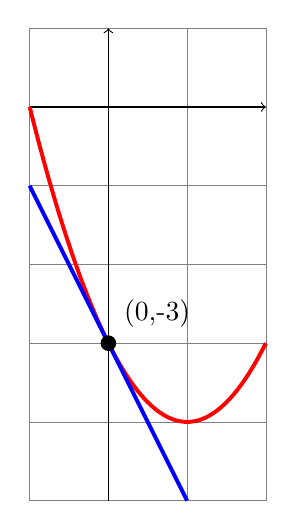
\begin{tikzpicture}
        \draw[gray,very thin] (-1,-5) grid (2,1);
        \draw[->] (-1,0)--(2,0);
        \draw[->] (0,-5)--(0,1);
        \draw[color=red, line width = 0.50mm]   plot[smooth,domain=-1:2]
        (\x, {-3-2*\x+(\x)^2});
        \draw[color=blue, line width = 0.50mm]
        plot[smooth,domain=-1:1] (\x, {-3-2*\x});
        \node[label={45:{(0,-3)}},circle,fill,inner sep=2pt] at (0,-3) {};
      \end{tikzpicture}
      \caption{Graphs of $y=x^2-2x-3$ and $y=-2x-3$}
      \label{fig:graphParabola}
    \end{figure}
  \end{enumerate}
\item %2
  \begin{enumerate}
  \item %2a
    We have
    \begin{align*}
      f(x+h) &= \frac{1}{x+h+1} \\
      f(x) &= \frac{1}{x+1} \\
      f(x+h)-f(x) &= \frac{1}{x+h+1} - \frac{1}{x+1} = \frac{(x+1) -
        (x+h+1)}{(x+h+1)(x+1)}
      = \frac{-h}{(x+h+1)(x+1)} \\
      \frac{f(x+h) - f(x)}{h} &= \frac{-1}{(x+h+1)(x+1)} \\
      f'(x) &= \lim_{h\to 0} \frac{f(x+h)-f(x)}{h} = \lim_{h\to 0}
      \frac{-1}{(x+h+1)(x+1)} = \frac{-1}{(x+1)^2}
    \end{align*}
    Substituting $x=0$,
    \begin{equation*}
      f'(0) = \frac{-1}{(0+1)^2} = -1
    \end{equation*}
    Using point-slope form, the equation of the tangent line is
    \begin{equation*}
      y - y_0 = m(x-x_0) \implies y - 1 = (-1) (x-0) \implies y - 1 =
      -x \implies y = -x + 1
    \end{equation*}
  \item %2b
    We have
    \begin{align*}
      f(x+h) &= \sqrt{2(x+h)-1} \\
      f(x) &= \sqrt{2x-1} \\
      f(x+h) - f(x) &= \sqrt{2(x+h)-1} - \sqrt{2x-1} \\
      \frac{f(x+h) - f(x)}{h} &= \frac{\sqrt{2(x+h)-1} -
        \sqrt{2x-1}}{h} \\
      f'(x) &= \lim_{h\to 0} \frac{f(x+h) - f(x)}{h} = \lim_{h\to 0}
      \frac{\sqrt{2(x+h)-1} - \sqrt{2x-1}}{h}
    \end{align*}
    To evaluate limits like this, multiply by the conjugate radical:
    \begin{align*}
      f'(x) &= \lim_{h\to 0} \frac{\sqrt{2x+2h-1} - \sqrt{2x-1}}{h}
              \times \frac{\sqrt{2x+2h-1} + \sqrt{2x-1}}{\sqrt{2x+2h-1} +
              \sqrt{2x-1}}
      \\
            &= \lim_{h\to 0} \frac{(2x+2h-1) -
              (2x-1)}{h(\sqrt{2x+2h-1}-\sqrt{2x-1})}
      \\
            &= \lim_{h\to 0} \frac{2h}{h(\sqrt{2x+2h-1}-\sqrt{2x-1})}
      \\
            &= \frac{2}{\sqrt{2x-1}+\sqrt{2x-1}} = \frac{2}{2\sqrt{2x-1}}
      \\
            &= \frac{1}{\sqrt{2x-1}}
    \end{align*}
    Substituting $x=5$ gives $f'(5) = 1/(2(5)-1) = 1/9$.  The equation
    of the tangent line is $y-3 = 1/9(x-5)$, which can be rearranged
    to $y=(1/9) x - 22/9$.
  \item %2c
    We have
    \begin{align*}
      f(x+h) &= (x+h)^3 - 4(x+h) = x^3 + 3x^2 h + 3xh^2 + h^3 - 4x -
      4h \\
      f(x) &= x^3 - 4x \\
      f(x+h) - f(x) &= 3x^2 h + 3xh^2 + h^3 - 4h \\
      \frac{f(x+h) - f(x)}{h} &= \frac{3x^2h + 3xh^2 - h^3 - 4h}{h} =
      3x^2 + 3xh - h^2 - 4 \\
      f'(x) &= \lim_{h\to 0} \frac{f(x+h)-f(x)}{h} = \lim_{h\to 0}
      3x^2 + 3xh - h^2 - 4 = 3x^2 - 4
    \end{align*}
    At $x=-1$, $f'(-1) = 3(-1)^2 - 4 = 3 -4 = -1$.  The equation of
    the tangent line is $y-3 = (-1)(x-(-1))$ or $y-3 = -x -1$ or
    $y=-x+2$.
  \item %2d
    We have
    \begin{align*}
      f(x+h) &= \frac{(x+h)^2}{2(x+h)-1} = \frac{x^2+2xh+h^2}{2x+2h-1}
      \\
      f(x) &= \frac{x^2}{2x-1} \\
      f(x+h) - f(x) &= \frac{x^2+2xh+h^2}{2x+2h-1} - \frac{x^2}{2x-1}
                      = \frac{(x^2+2xh+h^2)(2x-1)-(2x+2h-1)x^2}{(2x+2h-1)(2x-1)}
                      \\
                      &= \frac{2x^3 - x^2 + 4x^2h - 2xh + 2xh^2 - h^2 - 2x^3 - 2x^2h +
                        x^2 }{(2x+2h-1)(2x-1)} 
                        = \frac{4x^2h-2xh-h^2}{(2x+2h-1)(2x-1)} \\
      \frac{f(x+h) - f(x)}{h} &= \frac{4x^2h-2xh-h^2}{(2x+2h-1)(2x-1)}
                                = \frac{4x^2 - 2x -h}{(2x+2h+1)(2x-1)} \\
      f'(x) &= \lim_{h\to 0} \frac{4x^2 - 2x - h}{(2x+2h-1)(2x-1)}
      = \frac{4x^2 - 2x}{(2x-1)(2x-1)} = \frac{4x^2-2x}{(2x-1)^2}
    \end{align*}
  \end{enumerate}
\item %3
  \begin{enumerate}
  \item We have
    \begin{align*}
      f(a+h) &= 10 + 3(a+h)^2 - (a+h)^3 = 10 + 3a^2 + 6ah + 3h^2
               - a^3 - 3a^2h - 3ah^2 - h^3 \\
      f(a) &= 10 + 3a^2 - a^3 \\
      f(a+h)-f(a) &= 10 + 3a^2 + 6ah + 3h^2
                    - a^3 - 3a^2h - 3ah^2 - h^3 - 10 - 3a^2 + a^3 \\
             &= 6ah + 3h^2 - 3a^2h - 3ah^2 - h^3 \\
      \frac{f(a+h)-f(a)}{h} &= \frac{6ah+3h^2-3a^2h-3ah^2-h^3}{h}
    \end{align*}
    Taking the limit,
    \begin{align*}
      f'(a) &= \lim_{h\to 0} \frac{f(a+h)-f(a)}{h} \\
            &= \lim_{h\to 0} \frac{6ah+3h^2-3a^2h-3ah^2-h^3}{h} \\
            &= \lim_{h\to 0} (6a + 3h - 3a^2 - 3ah - h^2) \\
            &= 6a - 3a^2
    \end{align*}
  \item Now that we have a formula for the slope of the tangent line,
    we can apply it to obtain the slope immediately in both cases.  In
    the first case,
    \begin{displaymath}
      m = f'(1) = 6(1) - 3(1)^2 = 6 - 3 = 3
    \end{displaymath}
    so the point-slope form of the tangent line is
    \begin{displaymath}
      y - 12 = 3(x-1)
    \end{displaymath}
    You can further simplify your answer but that is not necessary.
    In the second case,
    \begin{displaymath}
      m = f'(3) = 6(3) - 3(3)^2 = 18 - 27 = -9
    \end{displaymath}
    so the point-slope form of the tangent line is
    \begin{displaymath}
      y - 10 = -9(x-3)
    \end{displaymath}
  \item See Figure~\ref{fig:graphCubic}.
    \begin{figure}[htbp]
      \centering
      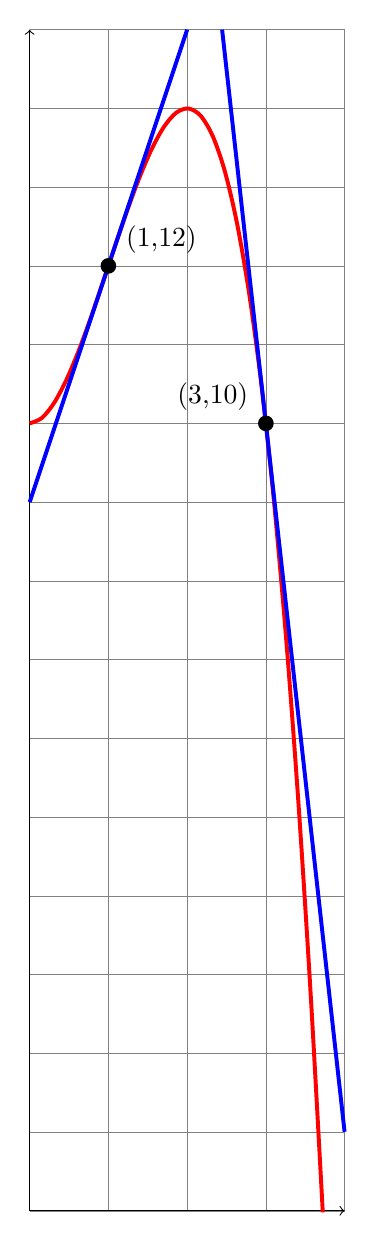
\begin{tikzpicture}
        \draw[gray,very thin] (0,0) grid (4,15);
        \draw[->] (0,0)--(4,0);
        \draw[->] (0,0)--(0,15);
        \draw[color=red, line width = 0.50mm]   plot[smooth,domain=0:3.723]
        (\x, {10+3*(\x)^2-(\x)^3});
        \draw[color=blue, line width = 0.50mm]
        plot[smooth,domain=0:2] (\x, {3*\x+9});
        \draw[color=blue, line width = 0.50mm]
        plot[smooth,domain=2.4444:4] (\x, {-9*\x+37});
        \node[label={20:{(1,12)}},circle,fill,inner sep=2pt] at (1,12) {};
        \node[label={160:{(3,10)}},circle,fill,inner sep=2pt] at (3,10) {};
      \end{tikzpicture}
      \caption{Graphs of $y=10+3x^2-x^3$ and $y=3x+9$ and $y=-9x+37$}
      \label{fig:graphCubic}
    \end{figure}
  \end{enumerate}
\item %4
  Instantaneous velocity is the derivative.  Since we need the
  velocity at several moments $t=1$, $t=2$, and $t=3$, we should find
  a general formula for the derivative.  We have
  \begin{align*}
    f(a+h) &= \frac{1}{a+h} \\
    f(a) &= \frac{1}{a} \\
    f(a+h)-f(a) &= \frac{1}{a+h} - \frac{1}{a} = \frac{a - a - h}{(a+h)(a)}
                  = \frac{-h}{(a+h)(a)} \\
    \frac{f(a+h)-f(a)}{h} &= \frac{-h}{(a+h)(a)(h)}
  \end{align*}
  Taking the limit,
  \begin{align*}
    v(a) = s'(a) &= \lim_{h\to 0} \frac{f(a+h)-f(a)}{h} \\
    &= \lim_{h\to 0} \frac{-h}{(a+h)(a)(h)} \\
    &= \lim_{h\to 0} \frac{-1}{(a+h)(a)} \\
    &= \frac{-1}{(a)(a)} \\
    &= \frac{-1}{a^2}
  \end{align*}
  Then at times $a=1$, $a=2$, and $a=3$ we have
  \begin{align*}
    v(1) &= \frac{-1}{1^2} = -1 \\
    v(2) &= \frac{-1}{2^2} = -\frac{1}{4} \\
    v(3) &= \frac{-1}{3^2} = -\frac{1}{9}
  \end{align*}
  where all velocity units are m/s.  Finally, the speeds are the
  absolute values of the velocities, so the speeds are
  \begin{align*}
    |v(a)| &= \left| -\frac{1}{a^2} \right| = \frac{1}{a^2} \\
    |v(1)| &= |-1| = 1 \\
    |v(2)| &= \left| -\frac{1}{4} \right| = \frac{1}{4} \\
    |v(3)| &= \left| -\frac{1}{9} \right| = \frac{1}{9}
  \end{align*}
  again in m/s.  Note that in $|v(a)|$ it is potentially tricky to get
  the sign right in general, but the fraction $1/a^2$ is always
  positive.
\item %5
  Note that there are many possible answers to this question.  First,
  we place a dot on an empty grid representing the point $(0,1)$
  through which the graph passes, and we draw a small line segment
  with slope $-1$ passing through the point $(0,1)$ representing the
  tangent line to the graph at the point.  See
  Figure~\ref{fig:four-conditions-1}(a).  Next, we draw a line segment
  of slope $0$ at a point $(1,y_1)$.  We are not given a condition on
  $y_1$ so we pick any $y_1$ (we should pick a value less than $1$ to
  get a nice graph).  See Figure~\ref{fig:four-conditions-1}(b).  We
  do the same thing with a small line segment of slope $3$ at the
  point $(2,y_2)$, where $y_2$ can be anything (but we should pick a
  value greater than $y_1$ to get a nice graph).  See
  Figure~\ref{fig:four-conditions-2}(c).  Finally, we sketch a nice
  smooth graph passing through the three points we have drawn, which
  is tangent to the three line segments we have drawn.  See
  Figure~\ref{fig:four-conditions-2}(d).
  \begin{figure}[htbp]
    \centering
    $\begin{array}{c@{\hspace{0.5in}}c}
    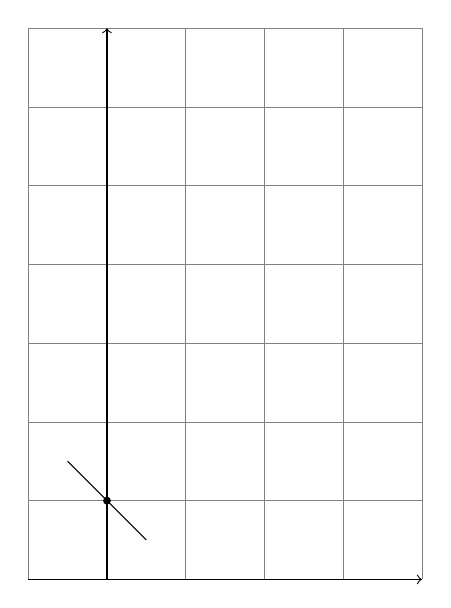
\begin{tikzpicture}[scale=1]
      \draw[gray,very thin] (-1,0) grid (4,7);
      \draw[->] (-1,0)--(4,0);
      \draw[->] (0,0)--(0,7);
      %\draw[color=red,domain=-1:3,samples=200] plot(\x,{(\x)^3/3-\x+1});
      \draw[color=black,domain=-0.5:0.5] plot(\x,{-\x+1});
      \fill[color=black] (0,1) circle (0.05);
      %\draw[color=black,domain=0.5:1.5] plot(\x,{1/3});
      %\fill[color=black] (1,1/3) circle (0.05);
      %\draw[color=black,domain=1.75:2.25] plot(\x,{3*(\x-2)+5/3});
      %\fill[color=black] (2,5/3) circle (0.05);
    \end{tikzpicture}
    &
    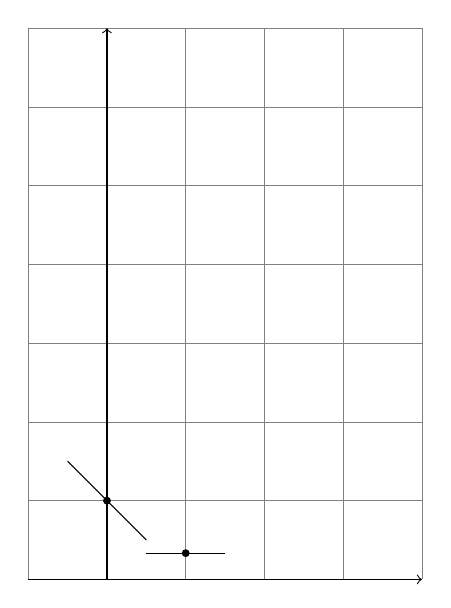
\begin{tikzpicture}[scale=1]
      \draw[gray,very thin] (-1,0) grid (4,7);
      \draw[->] (-1,0)--(4,0);
      \draw[->] (0,0)--(0,7);
      %\draw[color=red,domain=-1:3,samples=200] plot(\x,{(\x)^3/3-\x+1});
      \draw[color=black,domain=-0.5:0.5] plot(\x,{-\x+1});
      \fill[color=black] (0,1) circle (0.05);
      \draw[color=black,domain=0.5:1.5] plot(\x,{1/3});
      \fill[color=black] (1,1/3) circle (0.05);
      %\draw[color=black,domain=1.75:2.25] plot(\x,{3*(\x-2)+5/3});
      %\fill[color=black] (2,5/3) circle (0.05);
    \end{tikzpicture}
    \\
    \mbox{(a) Conditions $f(0)=1$, $f'(0)=-1$}
    &
    \mbox{(b) Adding condition $f'(1)=0$}
    \end{array}$
    \caption{First two conditions for graph}
    \label{fig:four-conditions-1}
  \end{figure}
  \begin{figure}[htbp]
    \centering
    $\begin{array}{c@{\hspace{0.5in}}c}
    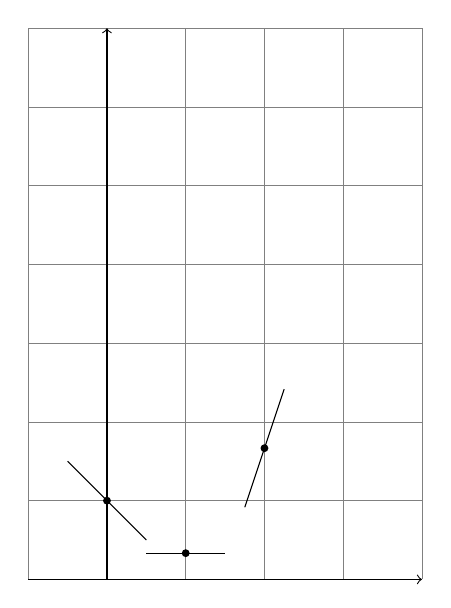
\begin{tikzpicture}[scale=1]
      \draw[gray,very thin] (-1,0) grid (4,7);
      \draw[->] (-1,0)--(4,0);
      \draw[->] (0,0)--(0,7);
      %\draw[color=red,domain=-1:3,samples=200] plot(\x,{(\x)^3/3-\x+1});
      \draw[color=black,domain=-0.5:0.5] plot(\x,{-\x+1});
      \fill[color=black] (0,1) circle (0.05);
      \draw[color=black,domain=0.5:1.5] plot(\x,{1/3});
      \fill[color=black] (1,1/3) circle (0.05);
      \draw[color=black,domain=1.75:2.25] plot(\x,{3*(\x-2)+5/3});
      \fill[color=black] (2,5/3) circle (0.05);
    \end{tikzpicture}
    &
    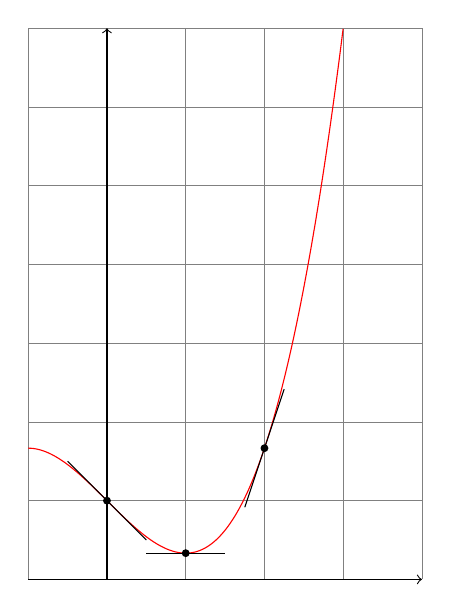
\begin{tikzpicture}[scale=1]
      \draw[gray,very thin] (-1,0) grid (4,7);
      \draw[->] (-1,0)--(4,0);
      \draw[->] (0,0)--(0,7);
      \draw[color=red,domain=-1:3,samples=200] plot(\x,{(\x)^3/3-\x+1});
      \draw[color=black,domain=-0.5:0.5] plot(\x,{-\x+1});
      \fill[color=black] (0,1) circle (0.05);
      \draw[color=black,domain=0.5:1.5] plot(\x,{1/3});
      \fill[color=black] (1,1/3) circle (0.05);
      \draw[color=black,domain=1.75:2.25] plot(\x,{3*(\x-2)+5/3});
      \fill[color=black] (2,5/3) circle (0.05);
    \end{tikzpicture}
    \\
    \mbox{(c) Adding Condition $f'(2)=3$}
    &
    \mbox{(d) Graph Consistent with (c)}
    \end{array}$
    \caption{Third Condition, and Graph Consistent with Conditions}
    \label{fig:four-conditions-2}
  \end{figure}
\item %6
  \begin{enumerate}
  \item We have
    \begin{align*}
      f(a+h) &= 4(a+h)^2 - (a+h)^3
               = 4a^2 + 8ah + 4h^2 - a^3 - 3a^2h - 3ah^2 - h^3 \\
      f(a) &= 4a^2 - a^3 \\
      f(a+h)-f(a) &= 4a^2 + 8ah + 4h^2 - a^3 - 3a^2 h - 3ah^2 - h^3 - 4a^2 + a^3
      \\
             &= 8ah + 4h^2 - 3a^2 h - 3ah^2 - h^3
    \end{align*}
    Taking limits of the difference quotient,
    \begin{align*}
      f'(a) &= \lim_{h\to 0} \frac{8ah+4h^2-3a^2h-3ah^2-h^3}{h} \\
            &= \lim_{h\to 0} (8a + 4h - 3a^2 - 3ah - h^2) \\
            &= 8a - 3a^2
    \end{align*}
  \item By the binomial theorem we have
    \begin{align*}
      f(a+h) &= (a+h)^4 - 5(a+h) = a^4 + 4a^3h+6a^2h^2+4ah^3+h^4-5a-5h \\
      f(a) &= a^4 - 5a \\
      f(a+h)-f(a) &= a^4 + 4a^3h + 6a^2h^2 + 4ah^3 + h^4 - 5a - 5h - a^4 + 5a \\
             &=4a^3h + 6a^2h^2 + 4ah^3 + h^4 - 5h
    \end{align*}
    Taking the limit of the difference quotient,
    \begin{align*}
      f'(a) &= \lim_{h\to 0} \frac{4a^3h + 6a^2h^2 + 4ah^3 + h^4 - 5h}{h} \\
            &= \lim_{h\to 0} (4a^3 + 6a^2 h + 4ah^2 + h^3 - 5) \\
            &= 4a^3 - 5
    \end{align*}
  \item We have
    \begin{align*}
      f(a+h) &= \frac{(a+h)^2 + 1}{a+h-2} = \frac{a^2+2ah+h^2+1}{a+h-2} \\
      f(a) &= \frac{a^2+1}{a-2} \\
      f(a+h)-f(a) &= \frac{a^2+2ah+h^2+1}{a+h-2} - \frac{a^2+1}{a-2} \\
             &= \frac{(a^2+2ah+h^2+1)(a-2)-(a^2+1)(a+h-2)}{(a+h-2)(a-2)} \\
             &= \frac{a^3 + 2a^2h + ah^2 + a - 2a^2-4ah-2h^2-2
               - a^3 - a^2h + 2a^2 - h + 2}{(a+h-2)(a-2)} \\
             &= \frac{a^2h + ah^2 - 4ah - 2h^2 - h}{(a+h-2)(a-2)}
    \end{align*}
    Taking the limit of the difference quotient,
    \begin{align*}
      f'(a) &= \lim_{h\to 0} \frac{a^2h+ah^2-4ah-2h^2-h}{h(a+h-2)(a-2)} \\
            &= \lim_{h\to 0} \frac{a^2 + ah - 4a - 2h - 1}{(a+h-2)(a-2)} \\
            &= \frac{a^2 - 4a - 1}{(a-2)^2}
    \end{align*}
  \item We have
    \begin{align*}
      f(a+h) &= \sqrt{3a + 3h + 1} \\
      f(a) &= \sqrt{3a+1} \\
      f(a+h)-f(a) &= \sqrt{3a + 3h + 1} - \sqrt{3a + 1}
    \end{align*}
    Taking the limit of the difference quotient and evaluating the
    limit by multiplying by the conjugate radical,
    \begin{align*}
      f'(a) &= \lim_{h\to 0} \frac{\sqrt{3a+3h+1}-\sqrt{3a+1}}{h} \\
            &= \lim_{h\to 0} \frac{\sqrt{3a+3h+1}-\sqrt{3a+1}}{h}
       \times \frac{\sqrt{3a+3h+1}+\sqrt{3a+1}}{\sqrt{3a+3h+1}+\sqrt{3a+1}} \\
     &= \lim_{h\to 0} \frac{(3a+3h+1)-(3a+1)}{h(\sqrt{3a+3h+1}+\sqrt{3a+1})} \\
            &= \lim_{h\to 0} \frac{3h}{h(\sqrt{3a+3h+1}+\sqrt{3a+1})} \\
            &= \lim_{h\to 0} \frac{3}{\sqrt{3a+3h+1}+\sqrt{3a+1}} \\
            &= \frac{3}{2\sqrt{3a+1}}
    \end{align*}
  \end{enumerate}
\item %7
  We have
  \begin{align*}
    y(t+h) &= 5(t+h) - 4.9(t+h)^2 = 5t + 5h - 4.9t^2 - 9.8 th - 4.9
             h^2 \\
    y(t) &= 5t - 4.9 t^2 \\
    y(t+h) - y(t) &= 5h - 9.8 th - 4.9 h^2 \\
    \frac{y(t+y)-y(t)}{h} &= 5 - 9.8 t - 4.9 h \\
    y' &= \lim_{h\to 0} \frac{y(t+h)-y(t)}{h} = \lim_{h\to 0}
         (5-9.8t-4.9h) = 5-9.8t
  \end{align*}
  At $t=0.5$ seconds, $y'(0.5) = 5-9.8(0.5) = 5-4.9 = 0.1$ meters per
  second.  Positive velocities are upward (and negative velocities
  would be downward) in this problem.
\item %8
  We have to figure out how to represent some of the numbers in the
  expressions differently.
  \begin{enumerate}
  \item Write $32=2^5$.  Then we have $f(x)=x^5$ and $a=2$.  Check.
  \item Write $4=\sqrt{16}$.  Then we have $f(x)=\sqrt{x}$ and
    $a=16$.  Check.
  %\item Write $1=e^0$.  Then we have $f(x)=e^x$ and $a=0$.  Check.
  \item Note that $\ds \sin \frac{\pi}{2} = 1$ so we can write the
    expression as
    \begin{displaymath}
      \lim_{t\to\pi/2} \frac{\sin t - \sin(\pi/2)}{t-\pi/2}
    \end{displaymath}
    which is an alternate form for the derivative of $f(t)=\sin t$ at
    $a=\pi/2$.
    
    Alternatively, you can convert the limit so it is a limit as
    $h\to 0$.  Let $h=t-\pi/2$, in which case $t=h + \pi/2$.  We have
    \begin{align*}
      \lim_{t\to\pi/2} \frac{\sin t - 1}{t-\pi/2}
      &= \lim_{h\to 0} \frac{\sin(h+\pi/2)-\sin(\pi/2)}{h}
    \end{align*}
    so we have $f(t)=\sin t$ and $a=\pi/2$.
  \end{enumerate}
\item %9
  In business applications, the derivative is usually interpreted
  as the ``marginal''.
  \begin{enumerate}
  \item The marginal cost is the cost of making one more widget after
    you have made $x$ widgets.  It can be written as
    \begin{equation*}
      f(x+1) - f(x) = \frac{f(x+1)-f(x)}{1} = \frac{f(x+h)-f(x)}{h}
    \end{equation*}
    where $h=1$.  If you are making large numbers of widgets, $1$ is
    considered close to $0$, so we have the approximation
    \begin{equation*}
      f'(x) = \lim_{h\to 0} \frac{f(x+h)-f(x)}{h} \approx
      \frac{f(x+1)-f(x)}{1}
    \end{equation*}
    so the derivative is approximately equal to the marginal.  The
    units are dollars per widget.
  \item $f'(100)=12$ means the cost of making one more widget, after
    you have already made 100 widgets, is 12 dollars.  (Usually the
    first few widgets are very expensive because they carry the fixed
    costs like renting factory space, etc.  After you get rolling, the
    cost of one more widget just includes the materials and labour,
    not the fixed costs.)
  \item For small values of $x$, the marginal cost will decrease as
    you make more widgets, because more of the fixed costs will be
    absorbed into the previously made widgets.  For large values of
    $x$ we may see an increase in the marginal cost because extra
    manufacturing capacity will need to be added beyond a certain
    level, and materials costs will increase because of the increasing
    demand caused by your manufacturing.
  \end{enumerate}
\item %10
  This question is hard.  When $x\ne 0$,
  \begin{align*}
    f(0+h) &= (0+h)^2 \cos \frac{1}{0+h}
    \\
    f(0) &= 0
  \end{align*}
  where we have used the first part of the definition of $f$ for
  values $x=0+h$ away from $0$, and the second part of the definition
  of $f$ for the value $x=0$.
  \begin{align*}
    \\
    f(0+h) - f(0) &= h^2 \cos \frac{1}{h}
    \\
    \frac{f(0+h)-f(0)}{h} &= h \cos \frac{1}{h}
    \\
    f'(0) &= \lim_{h\to 0} \frac{f(0+h)-f(0)}{h}
            = \lim_{h\to 0} h \cos \frac{1}{h}
  \end{align*}
  We have to be careful evaluating this limit.  We can't use the
  product rule for limits because
  \begin{equation*}
    \lim_{h\to 0} \cos \frac{1}{h}
  \end{equation*}
  does not exist.  Instead we have to use the squeeze theorem.  Note
  that $\cos$ is bounded between $-1$ and $1$:
  \begin{equation*}
    -1 \le \cos \frac{1}{h} \le 1
  \end{equation*}
  for any $h\ne 0$.  Assuming $h>0$, multiply by $h$ to obtain
  \begin{equation*}
    -h \le h \cos \frac{1}{h} \le h
  \end{equation*}
  Both $-h\to 0$ and $h\to 0$, squeezing the value in the middle, so
  we can conclude that the one sided limit
  \begin{equation*}
    \lim_{h\to 0^+} h \cos \frac{1}{h} = 0
  \end{equation*}
  You should make a similar (but slightly different) argument to show
  that $\lim_{h\to 0^-} h\cos (1/h) = 0$ also.  Since the one-sided
  limits exist and are equal, we conclude that
  \begin{equation*}
    f'(0) = \lim_{h\to 0} h \cos \frac{1}{h} = 0
  \end{equation*}
\end{enumerate}
\end{document}



%%%%%%%%%%%%%%%%%%%%%%%%%%%%%%%%%%%%%%%%%%%%%%%%%%%%%%%%%%%%%%%%%%%%%%
%%% MATH110-PS021-Solutions.tex ends here
